\documentclass{beamer}
\mode<presentation>
\usepackage{amsmath,amssymb,mathtools}
\usepackage{textcomp}
\usepackage{gensymb}
\usepackage{adjustbox}
\usepackage{subcaption}
\usepackage{enumitem}
\usepackage{multicol}
\usepackage{listings}
\usepackage{url}
\usepackage{graphicx} % <-- needed for images
\def\UrlBreaks{\do\/\do-}

\usetheme{Boadilla}
\usecolortheme{lily}
\setbeamertemplate{footline}{
  \leavevmode%
  \hbox{%
  \begin{beamercolorbox}[wd=\paperwidth,ht=2ex,dp=1ex,right]{author in head/foot}%
    \insertframenumber{} / \inserttotalframenumber\hspace*{2ex}
  \end{beamercolorbox}}%
  \vskip0pt%
}
\setbeamertemplate{navigation symbols}{}

\lstset{
  frame=single,
  breaklines=true,
  columns=fullflexible,
  basicstyle=\ttfamily\tiny   % tiny font so code fits
}

\numberwithin{equation}{section}

% ---- your macros ----
\providecommand{\nCr}[2]{\,^{#1}C_{#2}}
\providecommand{\nPr}[2]{\,^{#1}P_{#2}}
\providecommand{\mbf}{\mathbf}
\providecommand{\pr}[1]{\ensuremath{\Pr\left(#1\right)}}
\providecommand{\qfunc}[1]{\ensuremath{Q\left(#1\right)}}
\providecommand{\sbrak}[1]{\ensuremath{{}\left[#1\right]}}
\providecommand{\lsbrak}[1]{\ensuremath{{}\left[#1\right.}}
\providecommand{\rsbrak}[1]{\ensuremath{\left.#1\right]}}
\providecommand{\brak}[1]{\ensuremath{\left(#1\right)}}
\providecommand{\lbrak}[1]{\ensuremath{\left(#1\right.}}
\providecommand{\rbrak}[1]{\ensuremath{\left.#1\right)}}
\providecommand{\cbrak}[1]{\ensuremath{\left\{#1\right\}}}
\providecommand{\lcbrak}[1]{\ensuremath{\left\{#1\right.}}
\providecommand{\rcbrak}[1]{\ensuremath{\left.#1\right\}}}
\theoremstyle{remark}
\newtheorem{rem}{Remark}
\newcommand{\sgn}{\mathop{\mathrm{sgn}}}
\providecommand{\abs}[1]{\left\vert#1\right\vert}
\providecommand{\res}[1]{\Res\displaylimits_{#1}}
\providecommand{\norm}[1]{\lVert#1\rVert}
\providecommand{\mtx}[1]{\mathbf{#1}}
\providecommand{\mean}[1]{E\left[ #1 \right]}
\providecommand{\fourier}{\overset{\mathcal{F}}{ \rightleftharpoons}}
\providecommand{\system}{\overset{\mathcal{H}}{ \longleftrightarrow}}
\providecommand{\dec}[2]{\ensuremath{\overset{#1}{\underset{#2}{\gtrless}}}}
\newcommand{\myvec}[1]{\ensuremath{\begin{pmatrix}#1\end{pmatrix}}}
\let\vec\mathbf

\title{MatGeo Presentation - Problem 5.2.66}
\author{EE25BTECH11064 - Yojit Manral}
\date{}

\begin{document}

\frame{\titlepage}
\begin{frame}{Question}
Solve the system of equations
\begin{align}
    2x + 3y = 11 \\
    2x + 4y = -24
\end{align}
Hence, find the value of $m$ for which
\begin{align}
    y = mx + 3
\end{align}
\end{frame}

\begin{frame}{Solution}
$\rightarrow$ We have
\begin{align*} \vec{n_1}^T\vec{x} = c_1 && \vec{n_2}^T\vec{x} = c_2 \end{align*}
\begin{align} \implies \myvec{\vec{n_1}^T\\\vec{n_2}^T}\vec{x} = \myvec{c_1\\c_2} \end{align}
$\rightarrow$ From (1) and (2)
\begin{align}
    \vec{n_1} = \myvec{2\\3} && c_1 = 11 \\
    \vec{n_2} = \myvec{2\\4} && c_2 = -24
\end{align}
\end{frame}

\begin{frame}{Solution}
$\rightarrow$ From (4), (5) and (6)
\begin{align}
    \myvec{2&&3\\2&&4}\vec{x} = \myvec{11\\-24}
    &\xrightarrow{R_2 \leftrightarrow R_2 - R_1} \myvec{2&&3\\0&&1}\vec{x} = \myvec{11\\-35} \\
    &\xrightarrow{R_1 \leftrightarrow R_1 - 3R_2}\myvec{2&&0\\0&&1}\vec{x} = \myvec{116\\-35} \\
    &\xrightarrow{R_1 \leftrightarrow (1/2)R_1} \myvec{1&&0\\0&&1}\vec{x} = \myvec{58\\-35} \\
    &\implies \myvec{x\\y} = \myvec{58\\-35} \implies x = 58 \text{ and } y = -35
\end{align}
$\rightarrow$ From (3)
\begin{align}
    m = \frac{y - 3}{x} = -\frac{19}{29}
\end{align}
\end{frame}

\begin{frame}{Solution}
\begin{figure}[h!]
   \centering
   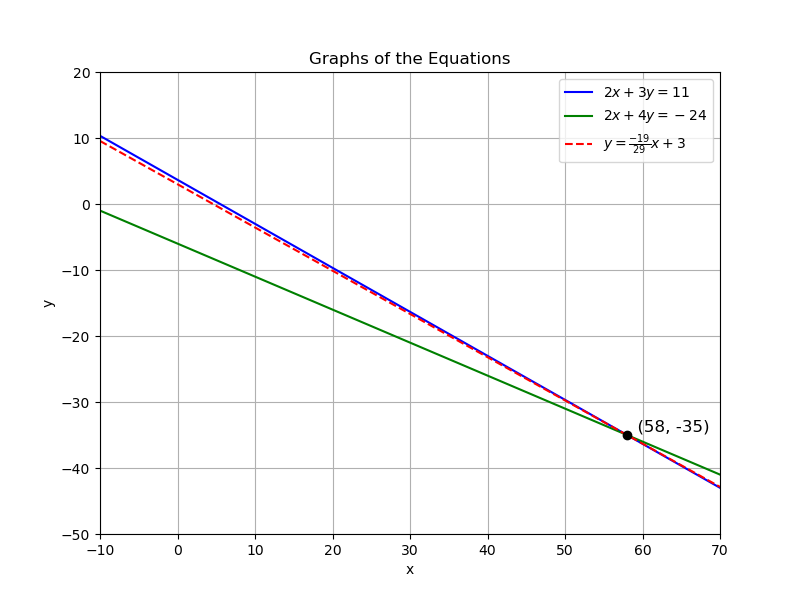
\includegraphics[width=0.7\linewidth]{figs/01.png}
   \caption{Plot of the Equations}
   \label{Plot_1}
\end{figure}
\end{frame}
 % --------- CODE APPENDIX ---------
\section*{Appendix: Code}
% Python plotting
\begin{frame}[fragile]{File: plot.py}
\begin{lstlisting}[language=Python]
import numpy as np
import matplotlib.pyplot as plt

# Define the x range
x_vals = np.linspace(-10, 70, 400)

# Equation 1: 2x + 3y = 11  --> y = (11 - 2x) / 3
y1_vals = (11 - 2 * x_vals) / 3

# Equation 2: 2x + 4y = -24  --> y = (-24 - 2x) / 4
y2_vals = (-24 - 2 * x_vals) / 4

# Line y = mx + 3 where m = -19/29
m = -19 / 29
y3_vals = m * x_vals + 3

# Plotting
plt.figure(figsize=(8, 6))

# Plot the lines
plt.plot(x_vals, y1_vals, label=r'$2x + 3y = 11$', color='blue')
plt.plot(x_vals, y2_vals, label=r'$2x + 4y = -24$', color='green')
plt.plot(x_vals, y3_vals, label=r'$y = \frac{-19}{29}x + 3$', color='red', linestyle='dashed')
\end{lstlisting}
\end{frame}

\begin{frame}[fragile]{File: plot.py}
\begin{lstlisting}[language=Python]
# Mark the point (58, -35)
plt.scatter(58, -35, color='black', zorder=5)
plt.text(58, -35, f'  (58, -35)', fontsize=12, verticalalignment='bottom')

# Set labels and title
plt.xlabel('x')
plt.ylabel('y')
plt.title('Graphs of the Equations')

# Show legend
plt.legend()

# Set axis limits for better viewing
plt.xlim(-10, 70)
plt.ylim(-50, 20)

# Show grid
plt.grid(True)

# Show plot
plt.show()
\end{lstlisting}
\end{frame}

\end{document}
